\documentclass[9pt,twocolumn,twoside]{styles/osajnl}
\usepackage{fancyvrb}
\journal{i524} 

\title{Apache Spark's Machine Learning Library (MLlib)}

\author[1]{Anvesh Nayan Lingampalli}


\affil[1]{School of Informatics and Computing, Bloomington, IN 47408, U.S.A.}


\affil[*]{Corresponding authors: anveling@umail.iu.edu}

\dates{\today}

\ociscodes{MLlib, Apache Spark, machine learning}

% replace this with your url in github/gitlab
\doi{\url{https://github.com/Anveling/sp17-i524/paper1/S17-IR-2016/report.pdf}}


\begin{abstract}
  This paper provides a summary about
  \href{https://spark.apache.org/docs/latest/ml-guide.html}{Apache
    Sparks Machine learning library (MLlib)} and its functionality.\newline
\end{abstract}

\begin{document}

\maketitle

\section{Introduction}

Apache Spark is a open source processing engine with consists of
elegant APIs, for performing efficient data analytics. It provides a
framework to process big data which are diverse in nature. Spark has
many advantages when compared to other technologies such as Hadoop and
Storm. Hadoop is also a big data processing technology which is proved
to be a solution for processing large data sets. But it is not
efficient in cases involving machine learning or streaming data. In
these cases, Hadoop requires other tools such as Mahout or Storm to
process the data. This is the most important advantage that the Apache
Spark has on Hadoop. Spark is faster in run times than Hadoop
MapReduce.\cite{MLlib-webpage}

\begin{figure}[htbp]
\begin{center}
\centering
\includegraphics[width= 2.5in]{images/hadoopvspark}
\caption{Hadoop vs Spark}
\label{fig:false-color}
\end{center}
\end{figure}

Spark in addition to Map and Reduce functions, also supports SQL
queries and machine learning. It has many libraries in Big Data
analytics and Machine Learning domains. MLlib is one of the top level
libraries that Spark offers.  MLlib (Machine Learning Library) is
Apache Spark’s scalable machine learning library with APIs in Java,
Python, R and Scala. It has the algorithms and tools for performing
various tasks on the data such as, clustering, classification,
regression and dimensionality reduction. The main goal of this library
is to make machine learning easy.

\section{History and Development}

Development of MLlib began in 2012 as a part of MLBase project (Kraska
et al., 2013). It is an open source since September 2013. It has since
then, been integrated into the Spark as an in-built package. The
original version of MLlib was developed in UC Berkeley and provided a
limited set of machine learning methods. Since it is an open source
community, MLlib developed and now has additional functionality.
 

\section{Components of MLlib}

MLib provides various linear models, Naive bayes and decision trees
for classification and regression problems. With the help of these
models, problems such as alternating least squares(ALS), k-means
problem, PCA (principal component analysis) for clustering have been
successfully implemented. Text mining, predictive analysis of data are
certain areas where MLlib is being used as an efficient tool.

MLlib has a package named spark.ml, which provides APIs for the
functionality of the pipelines. This package enables users to swap the
existing algorithms with their own algorithms.\cite{MLlib-article}

MLlib supports various methods for binary classification, multiclass
classification, and regression analysis. Each type of problem has its
own supported algorithms. Binary Classification has Linear SVMs,
Logistic regression, descision trees and naive Bayes. Multiclass
Classification also has decision trees and naive Bayes as its
supported algorithms. Regression has linear least squares, Lasso and
decision trees.

\section{Performance analysis between MLlib and its alternatives}
Hadoop Mahout is one of the alternative choice for a machine learning
library. Mahout uses Hadoop as underlying framework whereas in the
case of MLlib, it is Spark. In terms of features, support and
performance MLlib performs better. In 2014, Mahout announced it would
not accept Hadoop MapReduce and completely switched to Spark.

H2O, xgboost, python scikit-learn are few other alternatives to
MLlib. Scalability, speed and performance are measured for these tools
and are shown in the table below.

\begin{figure}[htbp]
\begin{center}
\centering
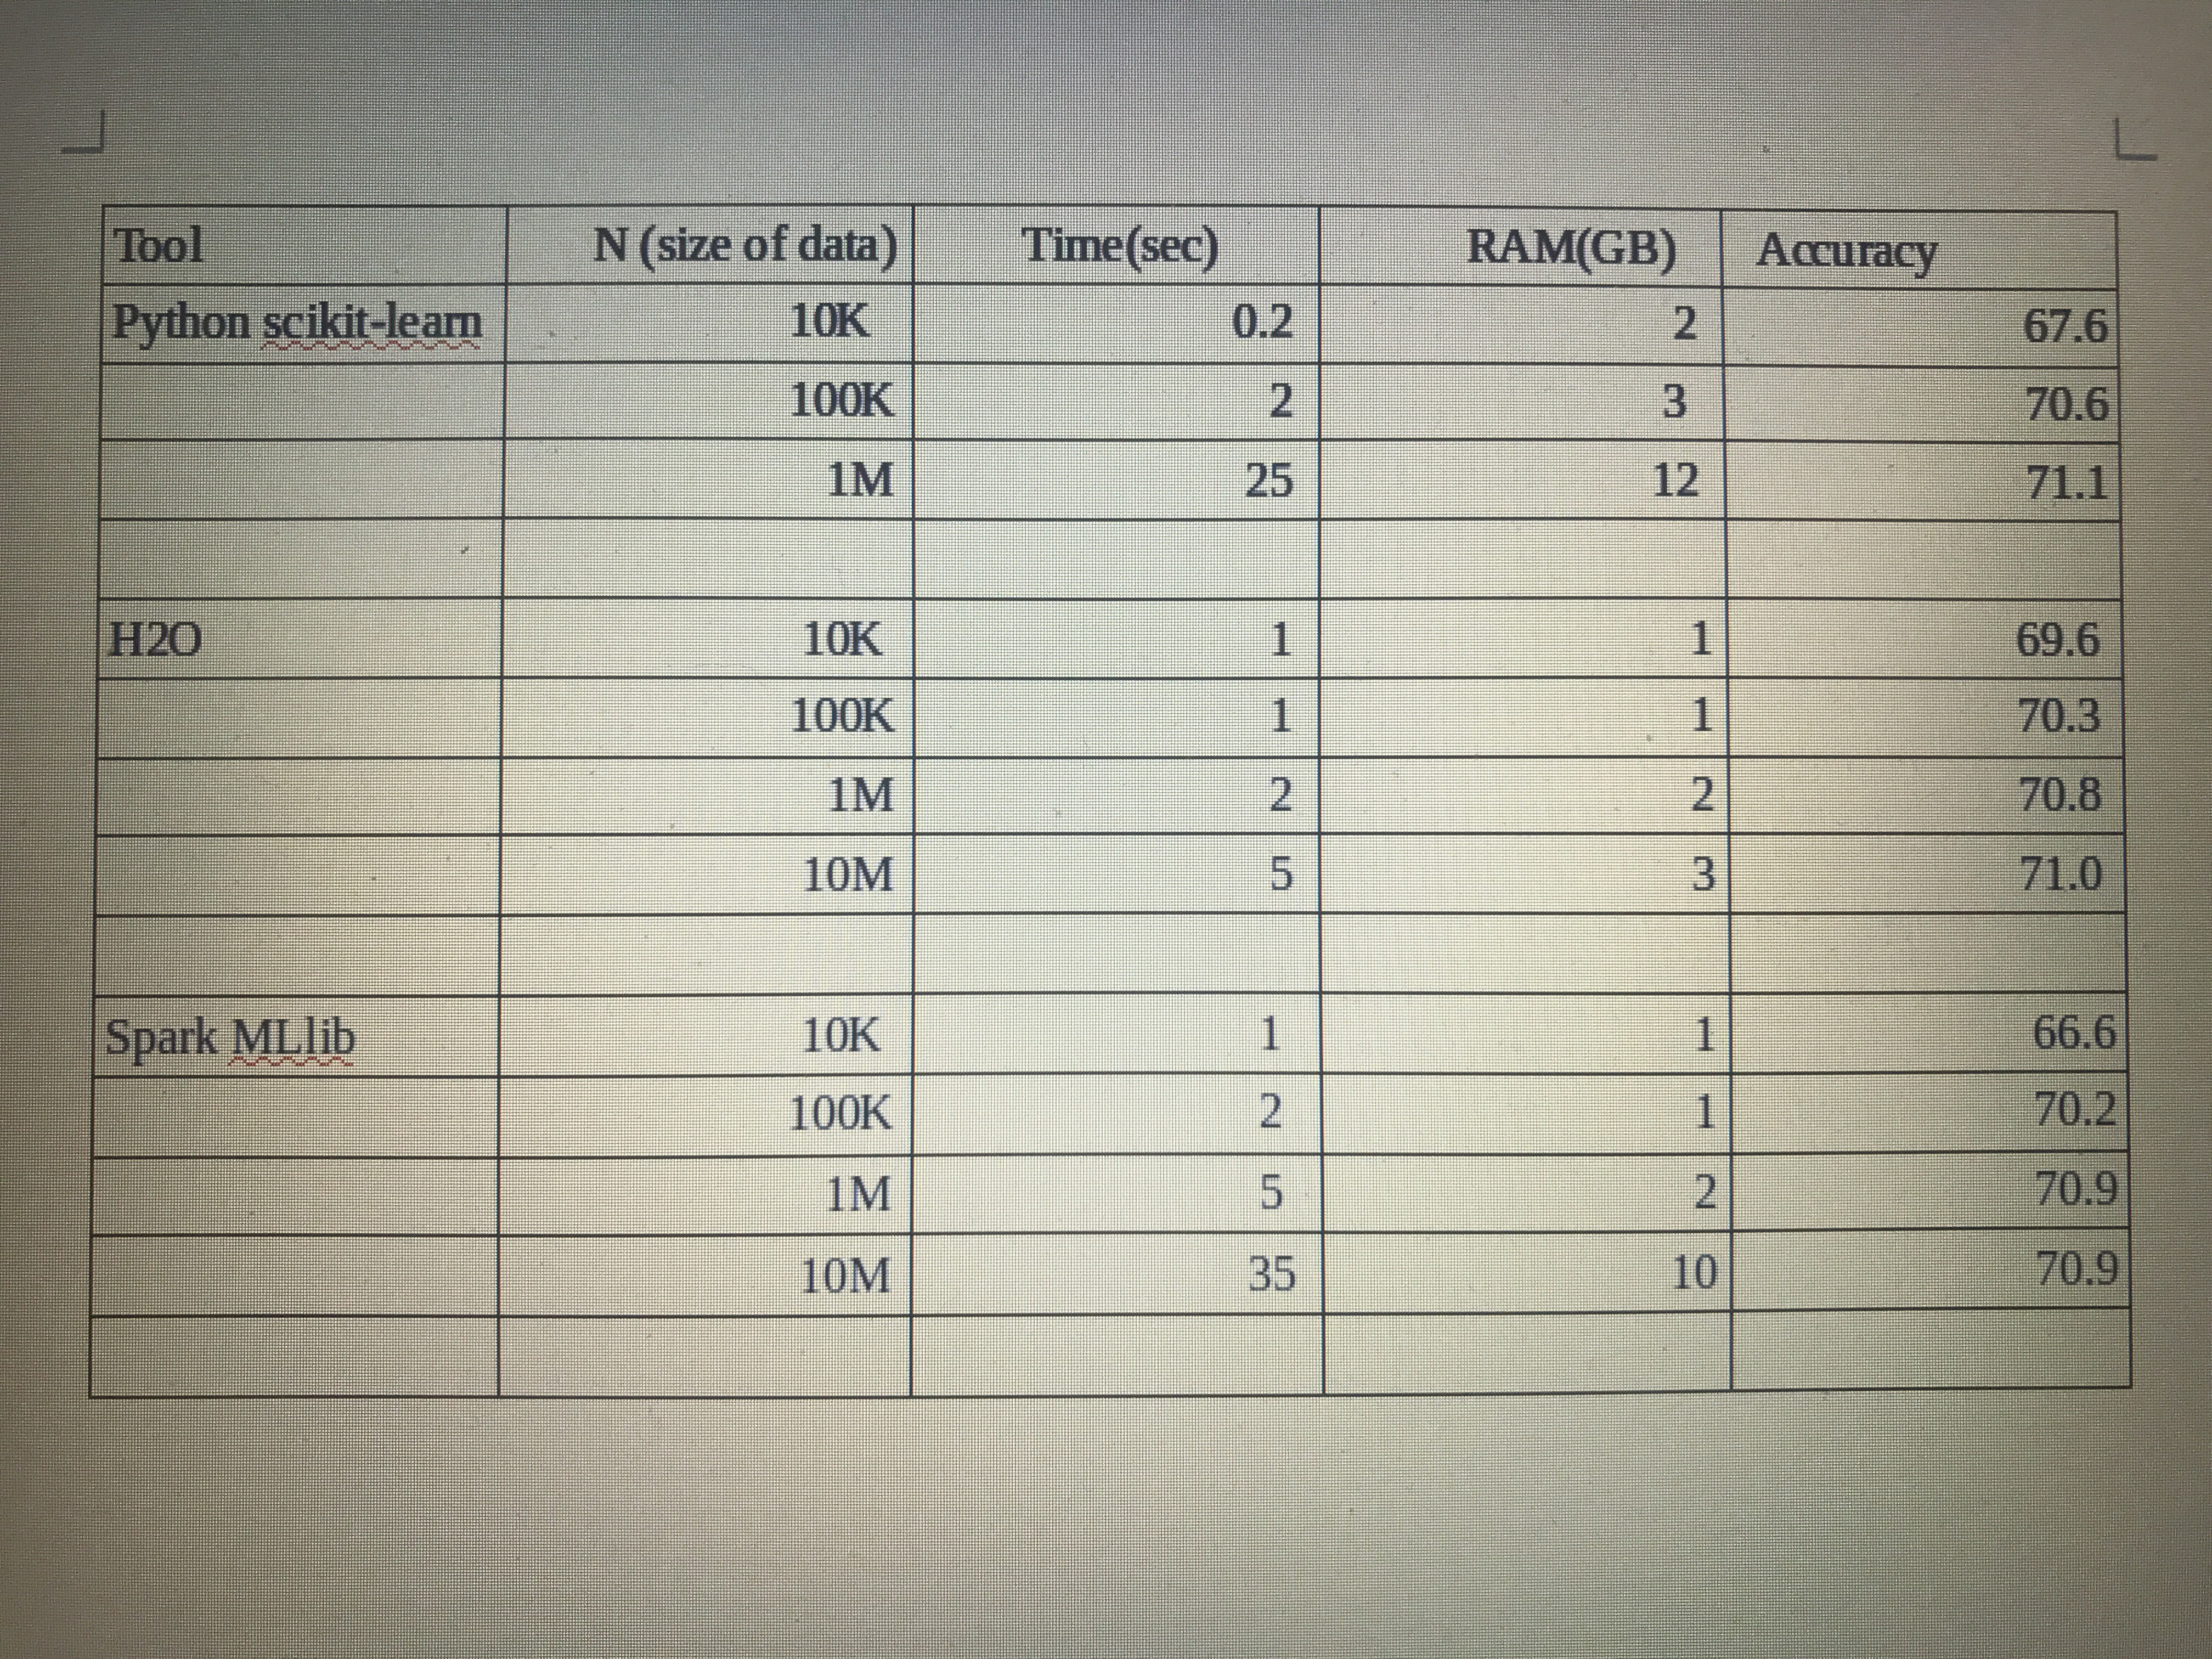
\includegraphics[width= \linewidth, height = 2.5in]{images/table1}
\caption{Analysis of performance}
\label{fig:false-color}
\end{center}
\end{figure}

For each tool and each size N, observations of the training tie,
memory usage, and accuracy are presented. These tests have been
carried out on a Amazon EC2 instance (32 cores, 60GB
RAM).\cite{Analysis-webpage}

The graph for the results is shown below. H2O is memory efficient and
faster than MLlib. But MLlib is the better choice of the two as it has
variety of functionalities.

\begin{figure}[htbp]
\begin{center}
\centering
\includegraphics[width=\linewidth]{images/analysisgraph}
\caption{Graph analysis}
\label{fig:false-color}
\end{center}
\end{figure}

\section{Use Cases}
Apache Spark Machine Learning Library is used in wide range of applications
in research and industry. Here two such applications are described
briefly.

\subsection{Movie Recommendation with MLlib}
In this mini course project MLlib library is used to make personalized
movie recommendations.\cite{Movie-Recommender}

\subsection{Predict Telco Churn with Apache Spark MLlib}

Churn prediction, is one of the most common applications of machine
learning in the telecommunications industry, as well as many other
subscriptions-based industries.MLlib is used here to fit a
machine-learning model that can predict which customers of a
telecommunications company are likely to stop using their
service.\cite{TelcoChurn}

\section{Useful Resources}

\cite{Machine-Learning-Library-(MLlib-Guide)-website} also
has some good step by step tutorials on how to use Machine learning
library to work on big data anlytics involving machine learning
learning studio.

\section{Conclusion}

In conclusion, MLlib is one of the best libraries to perform machine
learning as a part of big data analysis. It is still in active
development phase, and there have been many improvements over the
previous versions over time. MLlib provides developers with a wide
range of tools to make machine learning easy and scalable.

\section{Acknowledgements}

This work was done as part of the course "I524: Big Data and Open
Source Software Projects" at Indiana University during Spring
2017. 

\bibliography{references}

\end{document}
